Android is an open-source operating system (OS) developed by Google Inc., based on the Linux kernel and primarily designed for mobile touch-screen devices (e.g., smartphones, tablets, and watches). This chapter encompasses the structure of Android, such as the OS architecture and the BlueTooth LE protocol.

\subsection{Android Architecture}
The Android platform is an open-source and Linux-based software stack, containing six major components \cite{androidplatform} (as illustrated in \ref{fig:androidarhitecture}): 

\begin{figure}[h!]
    \centering
    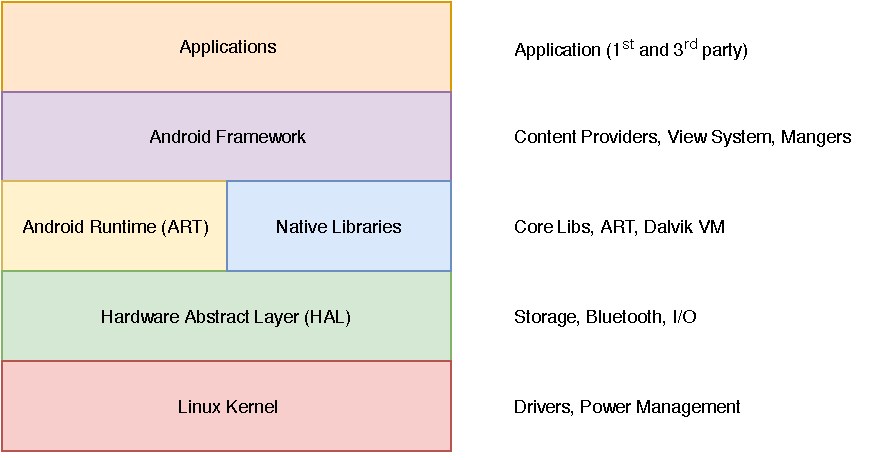
\includegraphics[scale=0.85]{images/Android.pdf}
    \caption{Android architecture stack, containing six major components.}
    \label{fig:androidarhitecture}
\end{figure}


\begin{description}
    \item[Applications:] Android provides a core set of applications (e.g., SMS, Mail, and browser) pre-installed on the device. There is support for installing third-party applications, which allows users to install applications developed by external vendors. A user is not bound to use the pre-installed applications for a service (e.g., SMS), and can choose the desired applications for service. Also, third-party applications can invoke the functionality of the core applications (e.g., SMS), instead of developing the functionality from scratch. 
    \item[Android Framework:] Is the building blocks to create Android applications by utilizing the core, all exposed through an API. The API enables reuse of core, modular system components, and services; briefly characterized as \textit{View System}: to build the user interface pre-defined components (e.g., lists, grids, and buttons); \textit{Resource Manager}: provides access to resources (e.g., strings, graphics and layout files); \textit{Notification Managers}: allows applications to show custom notifications in the status bar; \textit{Activity Manager}: manages lifecycle of the application; and \textit{Content Providers}: enables applications to access data from other applications.
    \item[Android Runtime:] Applications run in a seperate process and has its separate instance of the Android Runtime (ART). ART is designed to run on multiple virtual machines by executing DEX (Dalvik Executable format) files, which is a bytecode specifically for Android to optimize memory footprint. Some of the features that ART provides are ahead-of-time (AOT) and just-in-time (JIT) compilation, garbage collection (GC), and debugging support (e.g., sampling profiler, diagnostic exceptions, and crash reporting).
    \item[Native Libraries:] Most of the core Android components and services native code, that requires native libraries, is written in C or C++. The Android platform exposes Java APIs to some of the functionality of the native libraries (with Android NDK).   
    \item[Hardware Abstract Layer:] Provides an interface to expose hardware capabilities to the Java API framework. Hardware Abstract Layer (HAL) consists of multiple library modules that implement an interface for specific hardware components (e.g., camera, or BlueTooth module).
    \item[Linux Kernel:] is the foundation of the Android platform. The ART relies on the functionality from the Linux kernel, such as threading and low-level memory management. The Linux kernel provides drivers to services (e.g., BlueTooth, WiFi, and IPC), and incorporates a component for power management. 
\end{description} 



\subsection{Application Components}
Application components consist of four core components that are the building blocks of an Android application \cite{appfundamentals}. This section introduces these components; \verb|Activites|, \verb|Services|, \verb|BroadcastReceivers|, and \verb|Content Providers|. The activity is responsible for interactions with the user, services is a component that performs (long-running) tasks in the background, broadcast receivers handle broadcast messages from application components, and content providers manage shared set of application data. The Android system must be aware of the existence of the components, which can be accomplished by defining a manifest file (\verb|AndroidManifest.xml|) that describes the component and the interactions between them, as well as describe the permission of the application. 


\subsubsection{Activity}
An application can consist of multiple activities, and activity represents a single screen with a user interface \cite{activities}. Applications with multiple activities have to mark one of the activities as the main activity, which will be presented to the user on launch. The user interface of an activity is constructed in layout files which define the interaction logic of the user interface, and the layout file is inflated into the activity on launch. 

Activites are placed on a stack, and the activity on top of the stack becomes the running activity. Previous activities remain in the stack (unless disregarded), and are brought back if desired.  An activity can exist in three states cite[activites]:

\begin{itemize}
    \item \textbf{Resumed (Running)}: The activity is in the foreground of the screen and has user focus. 
    \item \textbf{Paused}: Another activity is running, but the paused activity is still visible. For instance, the other activity does not cover the whole screen. A paused activity maintains its state but can be killed by the system if the memory situation is critical.  
    \item \textbf{Stopped}: Another activity obscures the activity. A stopped activity maintains its state; however, it is not visible to the user and can be killed if the memory situation is critical.
\end{itemize}
Paused and stopped activities can be terminated due to insufficient memory by asking the activity to finish. When the paused or stopped activity is re-opened, it must be created all over. 

Activities are part of an activity lifecycle, in Figure \ref{fig:lifecycle}, the state of the activity can be vaguely categorized into:
\begin{itemize}
    \item \textbf{Entire Lifetime}: of an activity occurs between the calls to \verb|OnCreate()| and the call to \verb|OnDestroy()|. The activity sets the states (e.g., defining the layout) in \verb|OnCreate()|, and release remaining resources in \verb|OnDestroy()|.
    \item \textbf{Visible Lifetime}: of an activity happens between the calls to \verb|onStart()| and the call to \verb|onStop()|. Within this lifecycle, the user can see and interact with the application. Any resources that impact or affect the application occurs between these methods. As activities can alternative between state, the system might call these methods multiple times during the lifecycle of the activity.
    \item \textbf{Foreground Lifetime}: of an activity occurs between the calls to \verb|onResume()| and \verb|onPause()|. The activity is on top of the stack and has user input focus. An activity can frequently transition in this state; therefore, ensuring that the code in these methods is lightweight in order to prevent the user from waiting. 
\end{itemize} 

\begin{figure}
    \centering
    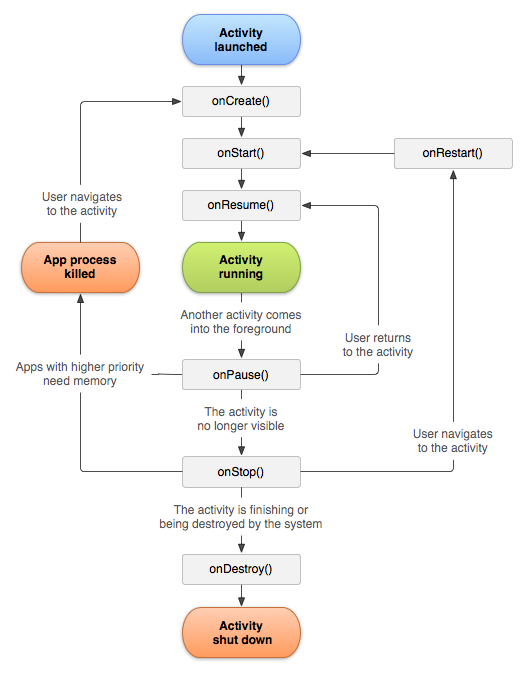
\includegraphics[scale=0.6]{images/androidlifecycle.png}
    \caption{Android activity lifecycle \cite{activities}.}
    \label{fig:lifecycle}
\end{figure}

\noindent \textbf{Fragment}

\noindent A fragment represents a behavior or is a part of a user interface that can be placed in an activity \cite{fragments}. Fragment allows for reuse of user interface or behavior across applications and can be combined to build a multi-pane user interface inside an activity. The fragment allows for more flexibility around the user interface, by allowing activities to comprise of multiple fragments which will have their own layout, events, and lifecycles. The lifecycle of a fragment is quite similar to the activity lifecycle; with extended states for fragment attachment/detachment, fragment view creation/destruction, and host activity creation/destruction. A fragment is coherent with its host activity, and the state of the fragment is affected by the state of the host activity. 

\subsubsection{Service}
Service is a component that runs in the background to perform long-running tasks \cite{services}. The application or other applications can start a service which remains in the background even if the user switches applications. In contrast, activities are not able to continue if the user switches to another application. Also, a service can bind with a component to interact or perform inter-process communication (IPC). To summarize, a service has two forms:
\begin{itemize}
    \item \textbf{Started}: A component can call the \verb|startService()| method on a service, such that the service can run in the background. 
    \item \textbf{Bound}: A component can call the \verb|bindService()| method on a service, which in return will offer a client-server interface to perform operations (e.g., sending requests, or retrieving results) across processes with inter-process communication (IPC). Multiple components can bind to a service, and the last component to \verb|unbind| will destroy the service. 
\end{itemize}

\subsubsection{Broadcast Receiver}
A broadcast receiver is a component that receives broadcast announcements mostly originating from the system (e.g., the screen turned off, the battery is low, or a picture was captured). Applications can subscribe to messages, and the \verb|BroadcastReceiver| can address and process the messages accordingly. Applications can also initiate broadcasts, and the data is delivered as an \verb|Intent| object. A \verb|BroadcastReceiver| can be registered in the activity of the application (with \verb|IntentFilter|), or inside of the manifest file. 

\subsubsection{Content Providers}
Content providers manage access to a set of structured data and provide a mechanism to encapsulate and secure the data \cite{contentproviders}. Content providers is an interface which enables one process to connect its data with another process. Also, in order to copy and paste complex data or files between applications, a content provider is required. For instance, to share a file across a media (e.g., mail), a \verb|FileProvider| (subclass of \verb|ContentProvider|) is needed to facilitate a secure sharing of files \cite{fileprovider}.


\subsection{Process and Threads}
The Android system creates a Linux process with a single thread of execution for an application on launch \cite{proccessandthread}. All components (i.e., activity, service, broadcast receiver, and providers) run in the same process and thread (called the \textit{main} thread) unless the developer arranges for components to run in a separate process. A process can also have additional threads for processing. 

When the memory on the device runs low and demanded by processes which are serving the user, Android might kill low priority processes. Android decides to kill the process based on priority; the process hierarchy consists of five levels (the lowest priority number is the most important and is killed last):  

\begin{enumerate}
    \item \textbf{Foreground Process}: is a process that is required by the user to interact and function with the application. A foreground process is  categorized as: activity that the user interacts with, service that is bound to an interacting activity, service that is running in the \verb|foreground| (with \verb|startForeground()|), service that is executing on of the lifecycle callbacks, and broadcast receivers executing \verb|onReceive()| method.
    \item \textbf{Visible Process}: is a process without foreground components, but affect the user interactions. A visible process is when a foreground process takes control (however, the visible process can be seen behind it), and a service that is bound to a visible (or foreground) activity. 
    \item \textbf{Service Process}: is a process that executes work which is not displayed to the user (e.g., playing music or downloading data), and are started with the \verb|startService()| method. 
    \item \textbf{Background Process}: is a process that holds information of paused activities. This process state has no impact on the user experience, and these processes are kept in an LRU (least recently used) in order to refrain killing the activity that the user used last. The state of the process can be saved if the lifecycle method in an activity is implemented correctly, to ensure seamless user experience. 
    \item \textbf{Empty Process}: is a process that does not hold any active application components; however, are kept alive for caching and faster startup time for components that need to be executed.  
\end{enumerate}


\noindent \textbf{Threads}

\noindent The main thread is responsible for dispatching events to the user interface widget and drawing events. Also, the thread interacts with the application components from the Android UI toolkit; the main thread is also called UI thread. System calls to other components are dispatched from the main thread, and components that run in the same process are instantiated from the main thread. Intensive work (such as long-running operations as network access or database queries) in response to user interaction, can lead to blocking of the user interface. As a consequence, the user can find the application to hang and might decide to quit or uninstall the application. 

Additionally, the tool kit to update the user interface in Android is not thread-safe; therefore, enforcing the rules of 1) not to block the UI thread; and 2) not to access the Android UI toolkit outside the UI thread. In order to run long-running or blocking operations, one can spawn a new thread or Android provides several options: \verb|runOnUiThread|, \verb|postDelay|, and \verb|AsyncTask| (perform an asynchronous task in a worker thread, and publishes the results on the UI thread). 

\subsection{Inter-Process Communication (IPC)}
Inter-process communication is a mechanism to perform remote procedure calls (RPC) to application components that are executed remotely (in another process), with results returned to the caller. To perform IPC, the caller has to bind to a remote \verb|service| (using \verb|bindService()|). Upon binding to a remote service, a proxy used for communication with the remote service is returned. The proxy decomposes the method calls, and the Binder framework takes the methods and transfers them to the remote process \cite{binder}. Android offers a language to enable IPC; called Android Interface Definition Language (AIDL) \cite{aidl}. 

Besides AIDL, one can use \verb|Intent| to pass messages across processes. The intent is a messaging object used to request action from other application components \cite{intents}. There are two types of intents: 1) \verb|explicit intents|: used to start a component in the application, by supplying the application package name or component class; and 2) \verb|implicit intents|: declare a general action to perform, which enables other applications to handle it. The main uses cases of intent are to starting an activity, starting a service, and delivering a broadcast.  

\subsection{Data and File Storage}
Android provides options to store application data on the device, depending on space requirement, data type, and whether the data should be accessible to other application or private to the application \cite{filestorage}. There are four distinctive data storage options, depending on the requirement of data that is being stored:
\begin{itemize}
    \item \textbf{Interal File Storage}: The system provides a directory on the file system for the application to store and access files. By default, the files saved in this directory is private to the application. Also, files stored in the internal storage are removed on uninstallation of the application; therefore, storing persistent data that are expected to be on the device regardless of the application removal, should not be using internal file storage. In addition, internal file storage allows for caching, which enables temporarily data storage (that do not require to be persistent). 
    \item \textbf{External File Storage}: External file storage enables storing of files in a space where users can mount to a computer as an external storage device (or to physical removable storage, such as SD card). Files stored into external storage makes it possible to transfer files on a computer over USB. Files stored in external file storage enables other applications to access the data, and the data remain available after application uninstallation (unless specified that the storage is application-specific). 
    \item \textbf{Shared Preferences}: For storing small and unstructured data, \verb|SharedPreference| enables API to read and write persistent key-value pairs of primitive data types (e.g., booleans, floats, ints, longs, and strings). The storage location is specified by uniquely identifying the name, and the data is stored into an XML file. Also, the data stored remain persistent (even after application termination). 
    \item \textbf{Databases}: Android provides support for SQLite databases, which is a relational database management system embedded in the system. The access to the database is private to the application, and accessing the database can be done with the \verb|Room persistence library|. The Room library provides an abstract layer over SQLite APIs.  
\end{itemize}


\subsection{Architecture Patterns}

\begin{figure}
    \centering
    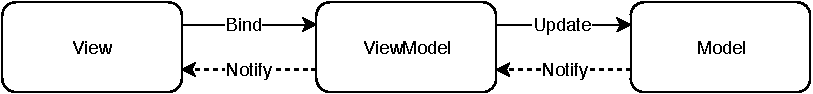
\includegraphics[scale=0.7]{images/MVVM.pdf}
    \caption{Structure of the Model-View-ViewModel architectural pattern.}
    \label{fig:mvvm}
\end{figure}

The architectural pattern principle enhances the separation of \textit{graphical user interface} logic from the \textit{oparting system} interactions \cite{architecture}. The Model-View-ViewModel (hereafter: MVVM) is an architectural pattern which is well-integrated in Android. It has three components that constitute the principle:
\begin{itemize}
    \item \textbf{Model}: represents the data and the business logic of the application. 
    \item \textbf{ViewModel}: interacts with the model, and manages the state of the view.
    \item \textbf{View}: handles and manages the user interface of the application.
\end{itemize}

In Figure \ref{fig:mvvm}, the interactions amongst the components are illustrated. The connection between the \verb|View| and \verb|ViewModel| occurs over a data binding connection, which enables the view to change automatically based on changes to the binding of the subscribed data \cite{mvvm}. In Android, the \verb|LiveData| is an observable data holder that enables data binding, which allows components to observe for data changes. \verb|LiveData| respects the lifecycle of the application components (e.g., activities, fragments, or services), ensuring the \verb|LiveData| only updates the components that are in an active lifecycle state \cite{livedata}. Moreover, \verb|Android Room| provides a set of components to facilitate the structure of the model component \cite{room}. More specifically, it models a database and the entities (which are the tables in the database).

\subsection{Power Management}
Battery life is a concern to the user, as the battery capacity is significantly limited on devices \cite{powermanagement}. Android has features to extend battery life by optimizing the behavior of the application and the device, and provides several techniques to improve battery life:
\begin{itemize}
    \item \textbf{App Restrictions}: Users can choose to restrict applications (e.g., applications cannot use the network in the background, and foreground services). The application that is restricted, functions as expected when the user launches the application; however, are restricted to do background tasks. 
    \item \textbf{App Standby}: An application can be put into standby mode if a user is not actively using it, resulting in the application background activity and jobs are postponed. An application is in standby mode if there is no process in the foreground, a notification is being viewed by the user, and not explicitly being used by the user. 
    \item \textbf{Doze}: When a device is unused for a long period, applications are delayed to do background activities and tasks. The doze-mode enters maintenance window to complete pending work, and then resume sleep for a longer period of time. This cycles through until a maximum of sleep time are reached. Some applications want to keep the device running to perform long-running tasks (e.g., collecting data), and \verb|WakeLocks| enables this. \verb|WakeLocks| allows the application to perform activities and tasks, even while the screen is turned off \cite{wakelocks}. 
    \item \textbf{Exemptions}: Another way of keeping an application awake, is to exempting applications from being forced to \verb|Doze| or in \verb|App Standby|. The exempted applications are listed in the settings of the device, and users can manually choose the application to exempt. Consequently, exempted applications might overconsume the battery of the device. 
\end{itemize}


\begin{figure}[h!]
    \centering
    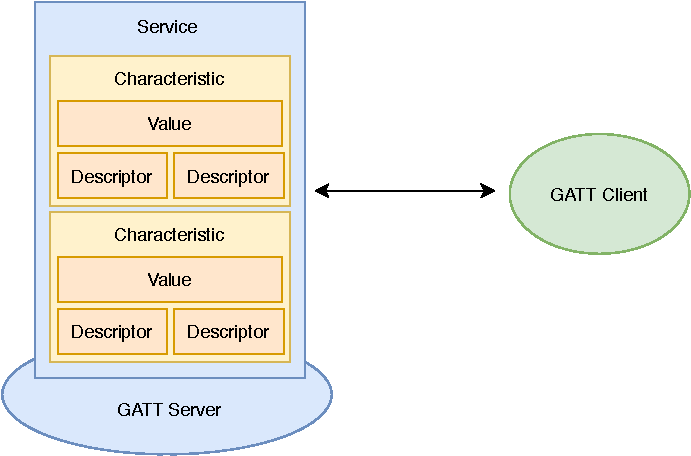
\includegraphics[scale=0.85]{images/BLE2.pdf}
    \caption{The structure of BlueTooth Low Energy; illustrating the GATT Server with a service containing many characteristics and its value, and the GATT client connecting with the GATT server.}
    \label{fig:BLE}
\end{figure}

\subsection{Bluetooth Low Energy}
Android supports for Bluetooth Low Energy (BLE), which is designed to provide lower power consumption on data transmission (in contrast to classic Bluetooth) \cite{bluetoothle}. BLE allows Android applications to communicate with sensors or devices (e.g., heart rate sensor, and fitness devices), that has stricter power requirements. Sensors that utilize BLE are designed to last for a longer period (e.g., weeks or months before needing to charge or replace battery). The protocol of BLE is optimized for a small burst of data exchange, and terms and concepts that form a BLE can be characterized as:
\begin{itemize}
    \item \textbf{Generic Attribute Profile (GATT)}: As of now, all Low Energy applications are based on GATT. GATT is a general specification for sending and receiving a burst of data (known as \textit{attributes}) over a BLE link. 
    \item \textbf{Attribute Protocol (ATT)}: GATT utilizes the Attribut Protocol, which uses a few bytes as possible to be uniquely identified by a Universal Unique Identifier (UUID). A UUID is a standardized format to identify information.
    \item \textbf{Characteristic}: Contains a single value and descriptors that describe the value of the characteristics (i.e., can be seen as a type). 
    \item \textbf{Descriptor}: Are defined attributes that describe a characteristic value (e.g., specify a human-readable description, a range of acceptable values, or a unit of measure).
    \item \textbf{Service}: Is a collection of characteristics (e.g., a service is \textit{Heart Rate Monitor} which includes a characteristic of \textit{heart rate measurement}).
\end{itemize}
In order to enable BLE, facilitating for a GATT server and GATT client is required. Either the sensor or the device takes the role of being a server or a client. However, the GATT server offers a set of services (i.e., features), where each service has a set of characteristics. Moreover, the GATT client can subscribe and read from the services the GATT server provides. 

